\documentclass[twocolumn,11pt]{article}
\usepackage{url}
\usepackage{graphics}
\usepackage{hyperref}
\usepackage{epsfig}
\usepackage{listings}
\usepackage{color}
\usepackage{amsmath}
\usepackage{amssymb}
\usepackage{graphicx}
\usepackage{subfigure}

\lstset{language=C}
\lstset{
    basicstyle=\ttfamily\small,
    keywordstyle=\color{blue},
    commentstyle=\color{green}
}
\newcommand{\chumma}[1]{\subsubsection {#1}}
\newcommand{\g}{\mathcal{G}}
\newcommand{\sql}[1]{{\tt \textbf{#1}}}
\newcommand{\wk}{\mathcal{W}}
\newcommand{\imgx}[2]{
	\begin{figure}[h]
	\centering
	\includegraphics[scale=0.6]{#1}
	\caption{#2}
	\end{figure}
}

\renewcommand{\topfraction}{0.9}	% max fraction of floats at top
\renewcommand{\bottomfraction}{0.8}	% max fraction of floats at bottom
%   Parameters for TEXT pages (not float pages):
\setcounter{topnumber}{2}
\setcounter{bottomnumber}{2}
\setcounter{totalnumber}{6}     % 2 may work better
\setcounter{dbltopnumber}{2}    % for 2-column pages
\renewcommand{\dbltopfraction}{0.9}	% fit big float above 2-col. text
\renewcommand{\textfraction}{0.07}	% allow minimal text w. figs
%   Parameters for FLOAT pages (not text pages):
\renewcommand{\floatpagefraction}{0.7}	% require fuller float pages
% N.B.: floatpagefraction MUST be less than topfraction !!
\renewcommand{\dblfloatpagefraction}{0.7}	% require fuller float pages


\title{\bf \textsf{CALF: Comparison of Attribute Layouts on Flash}}

\author{ Priyananda Shenoy \hspace{20pt} Satish Kumar Kotha \
\\
       {\em \normalsize Department of Computer Sciences}\\
       {\em \normalsize University of Wisconsin, Madison, WI}\\
       {\tt \normalsize \{shenoy,satish\}@cs.wisc.edu}}

\begin{document}
\date{}
\raggedbottom

\maketitle

\pagenumbering{arabic}
\pagestyle{plain}\setlength{\footskip}{25pt}

\begin{abstract}
\small
Solid state drives(SSDs) are increasingly being used for database applications, due to
their low seek latency and low power consumption. Solid state drives differ
fundamentally in their characteristics from disk drives, which mandates that
some core database design decisions, such as column layout, needs to take
into account the specific characteristics of SSDs for optimal performance.
This paper reexamines the question of column layout models for Flash based
databases. We propose a flexible data storage model which partitions attributes
based on a given workload, taking into account both reads and writes. We
evaluate the performance of this intelligent partitioning against NSM and C-Store
storage models.
\end{abstract}


\footnotetext{\small
	To appear in {\em DAWN'08: Proceedings of the First Database Aspects
	explored by Wisconsin's New researchers Conf.}, Dec 2-4, 2008. Madison, WI.\\
	Permission is not given to plagiarize this report for any class projects.
}

\section{Introduction}

In recent years, the cost-per-byte of Flash drives has fallen to an extent where
it is feasible to build fairly large applications on Flash storage. The lack of
mechanical parts, fast random access, low power consumption and durability are
some of the features which make it a storage medium of choice. While disk drives
will be around for a while, Flash has the potential to replace magnetic disks
in most applications.

As we will see in Section 3, Flash drives are inherently different from disk drives
in many respects. A significant number of architecture and design decisions behind
current database systems have (implicit or explicit) assumptions that work for
disk based systems, but not for Flash drives. In this paper, we explore the
decision of how columns of a relation are stored in secondary storage, and
examine how it can be optimized for Flash databases. Instead of statically
deciding column layout, we propose a way of coming up with a layout based on
a given workload.

\subsection{Organization of the paper}

Section 2 briefly introduces the various column-organization alternatives available.
Section 3 gives a short introduction to characteristics of Flash devices and how
they are different from disk drives. Section 4 gives the analytical cost modeling
of various operations. Section 5 describes our implementation and experimental setup.
Section 6 describes the results of evaluating the performance of our layout with
row, column based and CALF recommended page layouts.

\section{Related Work}

Column organization techniques can be roughly divided into two groups:
{\em Horizontal} or {\em row-major} storage models, where all attributes of a tuple
are stored together, and {\em Vertical} or {\em column-major} storage models
in which the data belonging to the same attribute are stored together.

The typical row-major storage model in use is the {\em N-ary Storage model}(NSM).
All the attributes of a tuple are laid out contiguously in a page. Each page
maintains a {\em slot table} which maintains the offset of the beginning of
each record. NSM is inefficient when only a few columns of the relation are
being accessed, since all the attributes are loaded irrespective of whether they
are used or not. CPU Cache performance is also bad, since loading unnecessary data
pollutes the cache.

{\em Decomposition Storage Model} (DSM) \cite{CK 85} was one of the first column-major
layouts. DSM split a $n$-column relation into $n$ sub-relations, duplicating
the primary key or record-id in each sub relation. This method saves on data
transfer when only a few columns are accessed, but pays a significant penalty
joining the relations when multiple attributes are accessed in the query.

{\em C-Store} \cite{SAB05} differs from DSM in that it doesn't explicitly store a
record-id per sub relation. C-Store maintains a collection of columns, where
an attribute of a column can be duplicated in multiple columns. Different columns
can store the same attribute values in different orders, which can help in
different queries.

{\em Partition Attributes Across}(PAX) \cite{ADH01} improves upon the cache behavior of NSM
by splitting a page into minipages, and storing the tuples in column-major order, each
column in one minipage. While this improves cache performance, this has no impact on
I/O transfer costs, since this just reorganizes data within a page, not across pages.

{\em Data Morphing}(DM) \cite{HP 03} improves upon the cache performance of PAX, by
making use of locality between attributes to group concurrently-accessed attributes
together. As with PAX, DM only optimizes in-page layout, and doesn't help in reducing
I/O transfer costs. This paper applies the same approach followed in DM to column
layouts across pages to reduce I/O transfer costs as well.

{\em Multiresolution Block Storage Model}(MBSM) \cite{ZR 03} extends the PAX model
to include multiple pages or blocks. Blocks are arranged to superblocks, which are
in turn grouped into Megablocks. Each block corresponds to a column. The relation
is partitioned onto multiple superblocks. This approach has good cache performance
and (somewhat) takes care of the data transfer problem. This model is no better
than column store in systems with inexpensive random reads, since most of the
organization is to make use of fast sequential access of disk drives.

There have been comparative studies of row-store vs. column-store organizations. 
Holloway et al. \cite{HD 08} found that in most read-heavy cases, column stores
beat row stores when I/O was the bottleneck. \cite{HBN06} also found similar
results, and proposed enhancing the row-storage model with some ideas
from column-storage. All these comparisons were for disk drives based databases,
hence the results may not hold true for Flash databases.

\cite{SHW08} briefly touches upon storage models for Flash, and mentions that
column-major layout is faster than row-major, for read queries. The authors also
touch upon the fact that write queries pose a problem for column major layouts,
incurring a heavy cost on inserts.

\section{Characteristics of Flash}

Flash drives have several traits that make them attractive for read-mostly
enterprise applications such as web-page serving and search. 
Flash drives are divided into blocks and each block is further divided into pages.
The memory can be read or programmed a byte or word in random access
fashion at a time but the unit of erasure is a block. Because of these 
characteristics, flash drives offer more random read I/Os per second, offer comparable
sequential bandwidth, and use a tenth of the power when compared to disks.
Flash is also cheaper than DRAM and is non-volatile. Moreover, flash
continues to get faster, cheaper, and denser at a rapid pace. However,
flash drives are limited by their write endurance. Flash memory cells
often wear out after 1000 to 10000 write cycles. Each write cycle requires
erasing a super block before writing the actual data. Techniques exist
to exploit wear levelling exist to extend the lifetime of the cells but
an overhead of remapping fragments is incurred and this technique is
useful only when there is a free super block available for the write.
Flash memory also allows multiple memory locations to be erased or
written in one programming operation and this is another major
advantage with respect to disks. Flash memories also have improved on reliability
which was one of it's major drawbacks during initial stages.

\section{Our Contribution}

We re-evaluate various storage models described in Section 2 for flash disks.
Much work so far has been focused on exploiting random reading offered by
flash disks. We also plan to focus on various workloads including writes
and analyze relative performance of various storage techniques. The next
section describes our cost model to start with and it has following
assumptions or limitations which we plan to get rid of as time
progresses.
\begin{itemize}
	\item There are no variable length attributes. For example, if datatype is defined
	as {\em varchar(255)}, we assume that it is implemented as fixed size of 255 bytes.
	\item Database application does not have control on how to write a random page. 
	Choosing an empty block instead of erasing and writing the block could minimize
	the costs associated. We consider average write cost in all our equations.
	\item No indexes on any of the columns. We plan to get rid of this assumption
	as early as possible, since it can have significant effect on the performance equations.
\end{itemize}

\subsection{Cost Modeling}

The key idea of Cost Modeling is to analytically estimate the cost of all operations in database for all possible layouts. Based on this cost model, we plan to organize the columns effectively in storage. Note that the cost model considers only bringing in pages from disk to memory. Some layouts may be cache-efficient and thus may improve performance, but we treat that as second order effect in our cost model.
Some definitions:
\begin{itemize}
\item $R$	  	: A relation in the database.
\item $A$	  	: The set of all columns of $R$ $\{a_1,a_2,\cdots,a_n\}$.
\item $sizeof(a_i)$ : The maximum number of bytes a column can take.
\item $G$	  	: A $group$ is a subset of columns $G \subseteq A$.
\item $\g$  	:	A $partition$ is a set of disjoint groups $\{G_1,G_2,\cdots,G_k\}$ such that $ \bigcup_{\g} G_i = A$.
\item $cost_r$: The cost to read a random page.
\item $cost_w$: The cost to write a random page.
\item $pagesize$: The number of bytes in a page.
\item $N$     : number of tuples in the relation.
\item $k$: Storage overhead per record in bytes. For example, in slotted page implementation, $k$ is slot table entry size.
\end{itemize}

The read and write costs are assumed to be constant. More details about how
these costs are estimated are given in Evaluation Section 6.1. Note that when
$|\g| = 1$, this would reduce to N-ary storage
model, and when $|\g| = |A|$, this reduces to column-store model.

The {\em records per page} for a group measures the number of tuples which
can be stored in one page, considering only the columns in that group.
\[ rpp(G) = \left\lfloor \frac{pagesize}{ \sum_{a \in G} sizeof(a) + k } \right\rfloor \]

To ensure that each page holds at least one record, we can impose the constraint
\[ \sum_{a \in G} sizeof(a) + k \leq pagesize. \]

For a given partition $\g$, the cost of a query depends on the type of query.
The cost calculations for each type of query is shown below.

\begin{itemize}
	\item $Q$ : \sql{select * from R}
	
	In this case, all the columns of the table are accessed for all rows.
	\[ cost(Q) =  cost_r \times \sum_{G \in \g} \left\lceil \frac{N}{rpp(G)} \right\rceil \].

	\item $Q$ : \sql{ select $s_1,s_2,\cdots,s_p$ from R}
	
	In this case, only some columns of the table are accessed for all
	rows. We incur a cost for a group if we access at least one attribute
	from it.
	\[ cost(Q) = cost_r \times \sum_{G \in \g} cost'(G,\{s_1,s_2,\cdots,s_p\}) \]
	where,
	\begin{align*}
	cost'(G,X) = \begin{cases}
		0 											&	X \cap G = \varnothing \\
		\left\lceil \frac{N}{rpp(G)} \right\rceil	&	otherwise
	\end{cases}
	\end{align*}
	
	\item $Q$ : \sql{select $s_1,s_2,\cdots,s_p$ from R where $p(w_1,w_2,\cdots,w_q)$}
	where $p$ is a boolean predicate.
	
	In this case, the cost depends on the selectivity of the query.
	Let {\em row selectivity} of a predicate be defined as
	\[ rowsel(p) = Pr_{tuple\;r \in R}\left[ p(r) = true \right]. \]
	Assuming that the distribution is uniform, the probability that
	none of the tuples in a given page belonging to a group $G$ match
	the predicate is given by $(1-rowsel(p))^{rpp}$. Hence the
	probability that at least one of the tuples in a page matches the predicate is
	$rowsel_G(p) = (1-(1-rowsel(p))^{rpp(G)})$. We incur a cost for
	a page if at least one record in that page matches the predicate.
	
	Then the cost of query $Q$ is
	\begin{align*}
		&cost(Q) = cost_r \times ( \sum_{G \in \g} cost''(G,W,S) ) \\
		&\text{where,} \\
		&cost''(G,W,S) = \\
		&\begin{cases}
			0			& G \cap W = G \cap S = \varnothing \\
			cost'(G,W)	& G \cap W \neq \varnothing \\
			cost'(G,S)  & G \cap W = \varnothing, G \cap S \neq \varnothing \\
			\times rowsel_G(p)
		\end{cases}
	\end{align*}
	
	\item $Q$: \sql{insert into R values($v_1,\cdots,v_n)$}
	
	For each group, we have to read the last page and see if there is
	space available. If not, we have to allocate a new page and insert
	the record there. In terms of I/O, we incur one page read and one
	page write for each insert operation.
	\[ cost(Q) = (cost_r + cost_w) \times |\g| \]
	
	\item $Q$: \sql{update table R set $s_1=v_1,\cdots,s_p=v_p$ where $p(w_1,\cdots,w_q)$}
	
	The cost calculation is similar to the select case seen above. We
	incur a read and a write cost for a page if there is at least one attribute
	in that group in the set clauses, and there is at least one
	record in that page which matches the predicate.
	
	\begin{align*}
		&cost(Q) = \sum_{G \in \g} cost_u''(G,W,S) \\
		&\text{where,} \\
		&cost_u''(G,W,S) = \\
		&\begin{cases}
			0				  									 	\\\hfill G \cap W  =   \varnothing, G \cap S  =   \varnothing \\
			cost_r \times cost'(G,W) & 							 	\\\hfill G \cap W \neq \varnothing, G \cap S  =   \varnothing \\
			rowsel_G(p) \times (cost_r + cost_w) \times cost'(G,S)  \\\hfill G \cap W  =   \varnothing, G \cap S \neq \varnothing \\
			(cost_r + rowsel_G(p) \times cost_w) \times cost'(G,W)  \\\hfill G \cap W \neq \varnothing, G \cap S \neq \varnothing \\
		\end{cases}
	\end{align*}
	
	\item $Q$: \sql{delete table R where $p(w_1,\cdots,w_q)$}
	
	Delete can be thought of as an update where every attribute needs
	to be updated (to a special `deleted' value). So the cost calculation
	is similar to the above case.
	\begin{align*}
		&cost(Q) = \sum_{G \in \g} cost_d''(G,W) \\
		&\text{where,} \\
		&cost_d''(G,W) = \\
		&\begin{cases}
			rowsel_G(p) \times cost_w \times cost'(G,A)				\\\hfill G \cap W  =   \varnothing \\
			(cost_r + rowsel_G(p) \times cost_w) \times cost'(G,W)	\\\hfill G \cap W \neq \varnothing
		\end{cases}
	\end{align*}
	
	Let $\wk = \{Q_i\}$ be a given workload. Then the {\em optimal partitioning} of
	a relation $R$ for the workload  is given by
	\[ \g_\wk^* = argmin_{\g} \sum_{Q_i \in \wk} cost_{\g}(Q_i). \]
\end{itemize}

\section{Implementation}

Our Implementation is broadly divided into three modules. 

\begin{itemize}
	\item Query Processing Engine:
	A Query Processing Engine converts standard sql format to CALF format. The main 
	difference between standard sql format and our format is adding selectivity as a 
	part of the query. Since we have not reached the level of doing predicate matching 
	and maintaining statistics about selectivity, we run the actual query on a 
	real database. Get selectivity of the query and use it to selectively read 
	pages. For example, sql query \sql{`update table $Table1$ set $column1 = 1$ where $column2 = 2$'}
	with four different equally likely values for column2 will be transformed to 
	CALF query \sql{`update $Table1$ 0.25 $column1:1$ $column2=2$'}. Note that the third 
	word in the CALF query is the selectivity.

	\item Optimal Partitioning Engine: 
	Given schema and workload, the goal of Optimal Partitioning Engine is to split the 
	columns into different groups in such a way that cost of workload according to the 
	CALF analytical model is minimum. This can be reduced to Minimum cost Set Partitioning
	problem and is NP-Hard. We use Branch and Bound technique as an approximation to 
	solve this problem. We start off by assuming table to have only one column. In this 
	case, all the layouts are equivalent. We then consider adding second column to the 
	table. There are two ways to do this. Put both the columns in same group or divide 
	them into two different groups. We compute cost for these two approaches and select 
	the best layout. The same approach is applied iteratively to reach final partition 
	with all the columns in the schema. The ideal algorithm would require $i!$ 
	comparisons in $i$th iteration while this approximation would require only $i$ 
	comparisons. But this approximation does not promise best possible partitioning. 
	However, it gives fairly good partitions as shown in previous subsections. We are 
	working on other better approximations to this problem that probably include domain 
	knowledge as a part of heuristic.

	\item Database Engine:
	The Database Engine consists of Storage module that takes responsibility of persisting 
	data and PageManager that interprets the stored data and helps in (un)marshalling of 
	data. We follow Slotted Page structure for all the layouts. Thus, Column layout for a 
	table with n-columns is actually stored as n-tables with one column each. We further 
	have some Meta information on attribute to page number mapping. This Meta information 
	helps in easily identifying the pages for a given group.

\end{itemize}

Figure 1 demonstrates the toolchain we developed for the evaluation.

\begin{figure}[htp]
	\begin{centering}
		\label{fig:case0}
		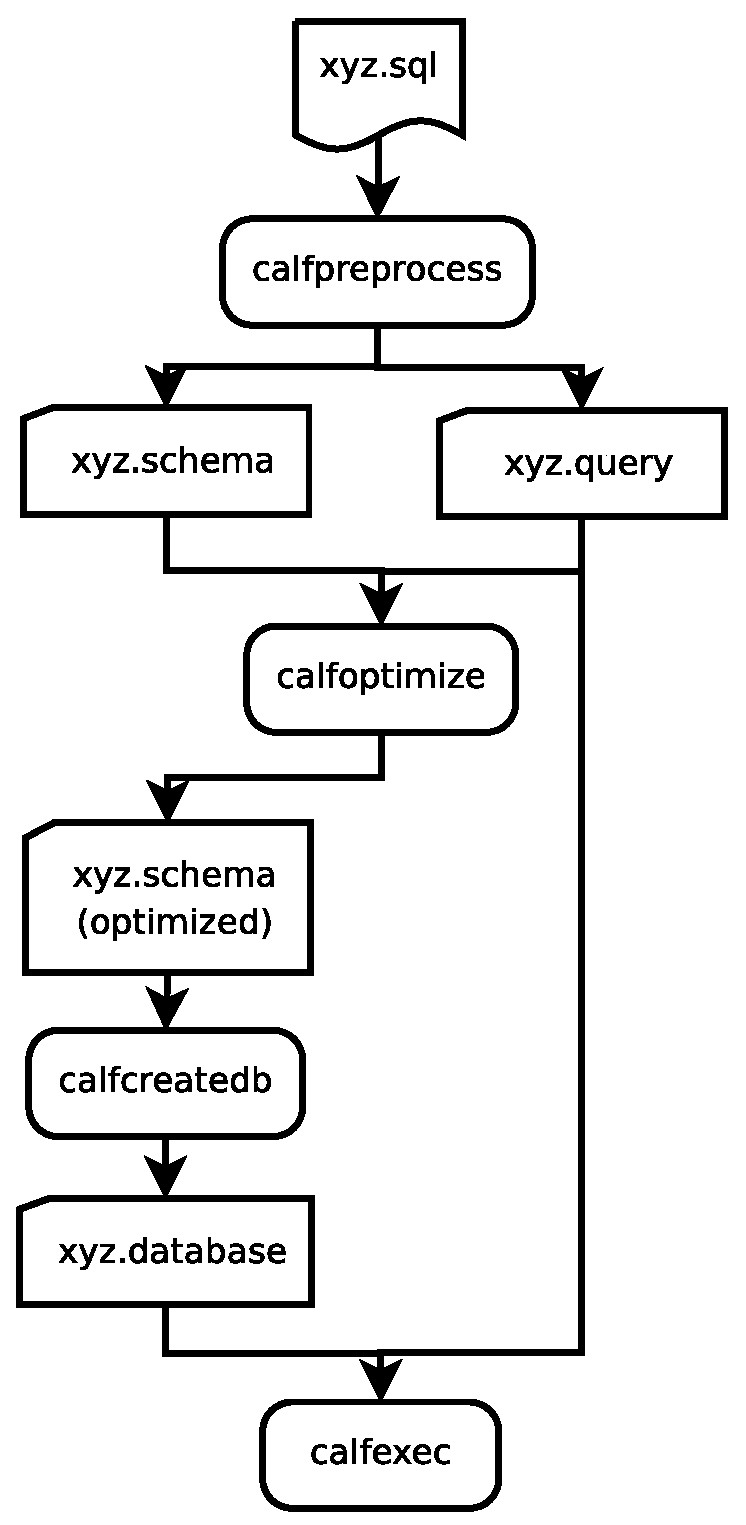
\epsfig{file=flow,width=120pt,height=240pt}
		\caption{Toolchain for evaluation}
	\end{centering}
\end{figure}

\begin{itemize}
	\item {\tt calfproprocess}: Converts SQL files into a simpler form which the 
	CALF engine can easily parse. It separates all the table creation statements
	into the schema file, and other statements into query files.
	\item {\tt calfoptimize}: Finds the optimal partitioning of attributes based
	on the analytical cost model.
	\item {\tt calfcreatedb}: Creates database files, which link the schema produced
	with specific column layout implementations.
	\item {\tt calfexec}: Executes the queries on the given database and measures
	the time it takes.
	\item {\tt calfblkload}: For initial loading of data into the database.
\end{itemize}
 
\section{Evaluation}

Our experimental setup was as follows:
\begin{itemize}
	\item Flash Device: Lenovo ChipsBnk 512MiB USB Stick over USB 2.0
	\item File  System: ext2
		\footnote{We planned to use a log-structured file system like logFS instead
		of a conventional file system, but practical difficulties getting logFS
		prevented us from doing so.}
	\item Operating system: Linux 2.6.27-2
	\item Page Size: 8KB
\end{itemize}

\subsection{Measurement of read/write costs on flash}

We measured the time taken to read and write one page from the file for
different page sizes. This is used as $cost_w$ and $cost_r$ in the Cost
Model calculations. We observed from our tests that random read and 
sequential read costs are equivalent. The following table shows the read
and write costs for various block sizes. As we have no control over the
actual erase operation, the erase costs are assumed to be amortized
over the write costs.\\

\begin{tabular}{|c|c|c|c|}
\hline
	{\small Page Size} 	& {\small Read time} & {\small Write Time}  & $\frac{write}{read}$\\
						& (ms)				 & (ms)					& \\
\hline
	8K 		  	& 20.117		& 111.192		 & 5.5637 \\
	16K			& 40.284		& 123.331		 & 3.0610 \\
	32K			& 82.392		& 138.815		 & 1.6767 \\
	64K			& 160.101		& 160.924		 & 1.0511 \\
\hline
\end{tabular}

As block size increases, the transfer cost begins to dominate the overall
cost of the operation, especially over a USB connection. We chose a page
size of 8K as a compromise between write-read ratio and the transfer rate.

\subsection{Layout comparison results}

We analyze a few workloads and see what our model predicts for row-store, column-store 
and CALF organizations. We then use the same workload and compare the results from actual 
CALF engine to our analytical model. For all the cases, we initially add 100,000 records 
to the database before executing the query that is being analyzed.

%\setlength{\parindent}{0in}
\renewcommand{\labelenumi}{\textbf{Case \arabic{enumi}}}

\begin{list}{\labelitemi}{\leftmargin=1em}{\rightmargin=10em}
	\item Cost of \sql{select * from R} while varying the number of attributes in $R$.
	
	\begin{figure*}[ht]
		\subfigure[Analytical model]{
			\epsfig{file=case1}
			\label{fig:case1}
		}
		\subfigure[On CALF Engine]{
			\epsfig{file=res1}
			\label{fig:res1}
		}
		\caption{\sql{select * from R}}
	\end{figure*}

	Figure \ref{fig:case1} shows the query cost using analytical model. Note that Optimal layout overlaps with 
	the Row layout. This is obvious because size of actual data stored and retrieved in both the 
	cases is same. But as the number of groups increase, the total slot table overhead increases 
	and therefore requires reading more pages. Thus, N-ary model outperforms all the other layouts.

	Figure \ref{fig:res1} shows the query cost by actually running the query on CALF database engine. The actual 
	results follow the results from analytical model. But, we observe a knee when number of columns 
	is a multiple of four. We attribute this to ratio of super block size (erase block size) to read 
	block size on the flash drive. 

	\item Cost of \sql{select $s_1,s_2$... from R} while varying the
	number of attributes in $R$, keeping the select clauses constant.

	\begin{figure*}[ht]
		\subfigure[Analytical model]{
			\epsfig{file=case2}
			\label{fig:case2}
		}
		\subfigure[On CALF Engine]{
			\epsfig{file=res2}
			\label{fig:res2}
		}
		\caption{\sql{select $s_1,s_2$ from R}}
	\end{figure*}

	Figure \ref{fig:case2} shows performance of various layouts when a subset of columns in the table are selected.
	The read cost for Row layout remains same as in Case 1 because all the pages are read into memory always.
	Column layout reads relatively more pages with small number of columns because of added storage overhead,
	but with increasing number of columns, it outperforms Row layout. The Optimal layout in this case divides
	$s_1$, $s_2$ into one group and all the remaining columns into the other. It thus reduces extra storage 
	overhead and reads only required data. Therefore, CALF predicts the best way to layout the columns.

	Figure \ref{fig:res2} shows the actual measured time for the same schema and query. This graph is
	approximately similar to the expected one, but the column costs are much higher than the row costs.
	The optimal is slightly worse than the row for the first few cases, but is stable as the number
	of columns increases.

	\item Cost of \sql{select $s_1,\cdots,s_k$ from R} while
	varying the number of attributes in the select clause, keeping the
	total number of attributes in $R$ constant(9).

	\begin{figure*}[ht]
		\subfigure[Analytical model]{
			\epsfig{file=case3}
			\label{fig:case3}
		}
		\subfigure[On CALF Engine]{
			\epsfig{file=res3}
			\label{fig:res3}
		}
		\caption{\sql{select $s_1,\cdots,s_k$ from R}}
	\end{figure*}

	Figure \ref{fig:case3} shows the analytical cost of the query as the number of
	attributes in the select clause is varied.
	The cost of Row layout remains constant because all pages are read in always. Cost with column 
	layout model increases linearly as expected as adding a new column in select clause requires 
	reading additional pages corresponding to that column. Again, the CALF Optimal layout selects 
	best partition of groups as the ones which contain exactly the same columns
	as those in the select clauses.

	Figure \ref{fig:res3} shows the actual measurement. The graph is close to expected
	value. The optimal one is slightly worse than the group one because of extra
	overhead.

	\item Cost of \sql{select $s_1,s_2$ from R where $p(w_1,w_2...)$}
	with varying selectivity of predicate $p$.

	\begin{figure*}[ht]
		\subfigure[Analytical model]{
			\epsfig{file=case4}
			\label{fig:case4}
		}
		\subfigure[On CALF Engine]{
			\epsfig{file=res4}
			\label{fig:res4}
		}
		\caption{\sql{select $s_1,s_2$ from R where $p(w_1,w_2...)$}}
	\end{figure*}

	Figure \ref{fig:case4} shows the analytical cost as the selectivity of
	$p$ is varied. This clearly shows a threshold phenomenon, since we
	read a page if at least one of the records in it match the predicate.
	We therefore skip a page only if the selectivity is $\approx \frac{1}{N}$.
	
	Figure \ref{fig:res4} shows the measured cost. In the absence of
	indices, our implementation reads all the where clause pages, which is why
	the sharp threshold is not seen in our implementation. Contrary to
	the model, column layout actually performs worse than the row one,
	again due to the extra overhead per record.
	
	\item Cost of \sql{update R $set s_1=v_1$... where p($w_1,w_2...$)}
	with varying selectivity of predicate $p$.

	\begin{figure*}[ht]
		\subfigure[Analytical model]{
			\epsfig{file=case5}
			\label{fig:case5}
		}
		\subfigure[On CALF Engine]{
			\epsfig{file=res5}
			\label{fig:res5}
		}
		\caption{\sql{update R set $s_1=v_1,...$ where p($w_1,w_2...$)}}
	\end{figure*}

	Figure \ref{fig:case5} shows the analytical cost of a fixed query as
	the selectivity of the predicate is varied. This is similar to the
	previous case, other than the fact that if the predicate matches there
	is an additional write cost.
	
	Figure \ref{fig:res5} shows the actual measurement. For reasons not 
	quite clear to us, there is significant variation in the timings. We suspect
	that it interleaved reads and writes is the cause of this. Also column
	and CALF are the ones which seem to be affected, which might indicate that
	non sequential writes are causing problems.

\end{list}

\section{Conclusions}
In this report, we analyze the cost of various storage models for a solid state device. 
We introduce an analytical model that decides on best partitioning of columns based on 
given workload. In general, analytical model points out that NSM performs better when 
there are relatively fewer columns because of added overhead in Column based approaches 
but as number of columns and tuples increase, Column layouts save lot of I/O.  We show 
that actual costs match the predictions of analytical model and CALF correctly predicts 
optimal partitioning of columns. Of course, CALF layout 
may incur high penalties because the queries chosen for partitioning
may not reflect the actual workload, and will not
work well for frequently changing workloads. We assume real workloads to have fairly 
predictable set of queries in the long run.

\section{Future work}
Several directions suggest themselves for future work. Obviously, fine-tuning cost model 
and improving it by considering database operations such as join and including other meta 
information such as indices on a column will be an ongoing task. We would also like to 
extend the database engine to variable length attributes and support more datatypes. 
Providing atomicity and consistency by implementing locking is also top on our list as 
this could be a serious disadvantage to column layouts. In addition, we also plan to 
address improvements to Optimal Partitioning approximation algorithm and consider the 
effect of number of records in database on the cost model.

\begin{thebibliography}{9999999}

\bibitem[GRA07]{GRA07} Goetz Graefe.
	The Five-minute Rule: 20 Years Later and How Flash Memory Changes the Rules.
	In {\em Proceedings of the Third International Workshop on Data Management on New Hardware}, 2007.
	
\bibitem[HD 08]{HD 08} Allison Holloway, David DeWitt.
	Read-Optimized Databases, In depth.
	In {\em $34^{th}$ International Conference on Very Large Data Bases}, 2008.

\bibitem[SHW08]{SHW08} Mehul Shah, Stavros Harizopoulis, Janet Wiener, Goetz Graefe.
	Fast Scans and Joins using Flash Drives.
	In {\em Proceedings of the Fourth International Workshop on Data Management on New Hardware}, 2008.

\bibitem[HP 03]{HP 03}
	Richard Hankins,Jignesh Patel.
	Data morphing: An adaptive,cache-conscious storage technique.
	In {\em Proceedings of the 29th VLDB Conference}, 2003.
	
\bibitem[ZR 03]{ZR 03}
	Jingren Zhou, Kenneth Ross.
	A Multi-resolution Block Storage Model for Database Design.
	In {\em Proceedings of the 2003 IDEAS Conference}, 2003.

\bibitem[SAB05]{SAB05}
	Mike Stonebraker, Daniel Abadi, Adam Batkin et al.
	C-Store: A Column-oriented DBMS.
	In {\em Proceedings of the 31st VLDB Conference}, 2005.

\bibitem[CK 85]{CK 85}
	George Copeland, Setrag Khoshafian.
	A decomposition storage model.
	In {\em Proceedings of the 1985 ACM SIGMOD international conference on Management of data}, 1985.

\bibitem[ADH01]{ADH01}
	A. Ailamaki, David DeWitt, Mark Hill, and M. Skounakis.
	Weaving relations for cache performance.
	In {\em Proceedings of VLDB Conference}, 2001.

\bibitem[HBN06]{HBN06}
	Alan Halverson, Jennifer Beckmann,Jeffrey Naughton,David DeWitt.
	A Comparison of C-Store and Row-Store in a Common Framework
	{\em Manuscript}, 2001.

\end{thebibliography}

\end{document}
